\documentclass[letterpaper,12pt]{article}
\usepackage[T1]{fontenc}
\usepackage[utf8]{inputenc}
\usepackage{lmodern}
\usepackage{amsmath}
\usepackage{cancel}
\usepackage{verbatim}
\usepackage{scrextend}
\usepackage{longtable}
\usepackage{framed}
\usepackage{amssymb}
\usepackage{wasysym}
\usepackage{multicol}
\usepackage{graphicx}
\usepackage{color}
\usepackage{caption}
\usepackage{subcaption}
\usepackage{float}
\usepackage{fancyhdr}
\usepackage[utf8]{inputenc}
\usepackage[mathletters]{ucs}
\usepackage{hyperref}
\usepackage{tikz,tkz-euclide}

\hypersetup
{
  colorlinks=false,
	pdfborder={0 0 0}
}

\title{Mathematical Foundations of Networking}

\pagestyle{fancy}

\begin{document}

\raggedright

\setlength{\columnseprule}{0.5pt}
\setcounter{tocdepth}{4}
\setcounter{secnumdepth}{6}
\tableofcontents

This book is separated into three parts. The first, are explanation of the
results, and informal proofs. The second part is the formula proof. The final
part is all the results enumerated.


\newpage
\newlength{\tmpparskip}
\setlength{\tmpparskip}{\parskip}
\setlength{\parskip}{-3mm}
\section{Results}
\subsection{Analytical Results}


\subsubsection{Single Server}

Let $\lambda$ be the arrival rate. Then the average inter-arrival time (time
between successive arrivals) is given by:
\begin{equation*} \begin{split}
	InterarrivalTime = \frac{1}{\lambda}
\end{split} \end{equation*}

Let $\mu$ be the the service rate. Then the average service time is given by:
\begin{equation*} \begin{split}
	ServiceTime = \frac{1}{\mu}
\end{split} \end{equation*}

The service time of a job is computed by:
\begin{equation*} \begin{split}
	ServiceTime = \frac{ServiceRequirement}{ServerCapacity}
\end{split} \end{equation*}

Let $n$ be the number of jobs that arrived in time period (0,L). \\
Assume that $n$ is also the number of jobs processed in time period (0,L). \\
Let $x_j$ be the service time of the $j^{th}$ job. \\
Let $Y$ be the throughput, the rate at which jobs are completed. Then
\begin{equation*} \begin{split}
	Y = \lambda = \frac{n}{L}
\end{split} \end{equation*}
Let $S$ be the mean service time. Then:
\begin{equation*} \begin{split}
	S = \frac{1}{n} \sum_{j=1}^n x_j
\end{split} \end{equation*}

Let $U$ be the utilization, the percentage of time that the server is busy.
Then:
\begin{equation*} \begin{split}
	U = \frac{1}{L} \sum_{j=1}^n x_j = \lambda S = Y S
\end{split} \end{equation*}

Let $r_j$ be the response time of the $j^{th}$ job. \\
Let $R$ be the mean response time. Then
\begin{equation*} \begin{split}
	R = \frac{1}{n} \sum_{j=1}^n r_j
\end{split} \end{equation*}
Let $Q$ be the mean number of jobs in the system. Then
\begin{equation*} \begin{split}
	Q = \frac{1}{L} \sum_{j=1}^n r_j = \lambda R = Y R \mbox{ (Little's Law) }
\end{split} \end{equation*}

\subsubsection{Open Network Model}

Let $p_{ij}$ be the probability goes from server i to server j after finishing at i. \\
The $(M+1)^{th}$ $p_{i,(M+1)}$ is the probability for leaving the system from server i. \\
The probability of take any of the edges when leaving a server $i$ is one, so:
\begin{equation*} \begin{split}
	\sum_{j=1}^{M+1} p_{ij} = 1 \; \forall i
\end{split} \end{equation*}
Let $\gamma_i$ be the arrival rate of jobs coming from outside the system.\\
The arrival rates at each server can be solved using the following equations (M
unknowns are the $\lambda_i$'s).
\begin{equation*} \begin{split}
	\lambda_i = \gamma_i + \sum_{j=1}^M \lambda_j p_{ji}
\end{split} \end{equation*}
Let $U_i$ be the utlization of server i. \\
Let $Q_i$ be the mean number of jobs at server i. \\
Let $R_i$ be the mean response time at server i. \\
Let $\gamma$ be the total arrival rate of jobs entering the system. \\
Let Y be the system throughput. \\
Let R be the system response time. Then:
\begin{align*} 
	U_i &= \lambda_i S_i \\
	Q_i &= \lambda_i R_i \\
	Q   &= \sum_{i=1}^M Q_i \\
	Y   &= \sum_{j=1}^M \lambda_i P_{i,(M+1)} = \sum_{i=1}^M \gamma_i \\
	R   &= \frac{Q}{\gamma} = \frac{1}{\gamma} \sum_{i=1}^M \lambda_i R_i
\end{align*} 



\subsubsection{Finite Population}

Let $N$ be the number of users. \\
Let $Z$ be the mean think time. \\
Recall that $S$ is the mean service time. \\
Recall that $L$ is the length of the observation period. \\
Recall that we assume $n$ is the number of jobs that enter equal to the number
that leave the system.
\begin{equation*} \begin{split}
	R = \frac{N}{Y-Z}
\end{split} \end{equation*}
We know that
\begin{equation*} \begin{split}
	U = YS \le 1
\end{split} \end{equation*}
So
\begin{align*}
	N^*  & = \frac{S+Z}{Z} \\
	R & \ge 
	\left\{
		\begin{alignedat}{3}
			& S     & \qquad & 1 \le  & N \le N^* \\
			& NS-Z  & \qquad &        & N  >  N^*
		\end{alignedat}
	\right. \\
	Y & \le
	\left\{
		\begin{alignedat}{3}
			& \frac{N}{S+Z} & \qquad & 1 \le  & N \le N^* \\
			& \frac{1}{S}   & \qquad &        & N  >  N^*
		\end{alignedat}
	\right.
\end{align*}

\subsubsection{Closed Network Model: No Users (ie: Cycle)}
Let $p_{ij}$ be the probability goes from server i to server j after finishing at i. \\
Notice there is no $p_{i,0}$ or $p_{i,(M+1)}$ \\
The probability of take any of the edges when leaving a server $i$ is one, so:
\begin{align*} 
	\sum_{j=1}^{M} p_{ij} = 1 \; \forall i
\end{align*} 
Recall $\lambda_i$ is the arrival rate of jobs at server i \\
We get the follow set if linearly {\bf dependant} :
\begin{align*} 
	\lambda_i = \sum_{j=1}^M \lambda_j p_{ji}
\end{align*} 
We can only determine:
\begin{align*} 
	\frac{\lambda_i}{\lambda_j} &= \frac{Y_i}{Y_j} \\
	\frac{U_i}{U_j} &= \frac{\lambda_i S_i}{\lambda_j S_j}
\end{align*} 
Let $U_b$ be the server with highest utilization. Then:
\begin{align*} 
	U_i \le \frac{\lambda_i S_i}{\lambda_b S_b}
\end{align*} 

\subsubsection{Closed Network Model: Web Application}
Let $p_{ij}$ be the probability goes from server i to server j after finishing at i. \\
The $0^{th}$ $p_{i,0}$ is the probability of the request returning to the user. \\
The probability to take any of the edges when leaving a server $i$ is one, so:
\begin{align*} 
	\sum_{j=0}^{M} p_{ij} = 1 \; \forall i
\end{align*}
We get the follow set if linearly {\bf dependant} :
\begin{align*} 
	\lambda_i = \sum_{j=0}^M \lambda_j p_{ji}
\end{align*} 
Let $V_i$ the the visit ration:
\begin{align*} 
	V_i = \frac{\lambda_i}{\lambda_0}
\end{align*} 
Let $D_i = V_i S_i$ (???) \\
The throughput of the system is total arrival rate from the users. This gives
us:
\begin{align*} 
	Y &= \lambda_0 \\
	\lambda_i &= Y V_i \\
	U_i &= \lambda_i S_i = Y V_i S_i = Y D_i \\
	\frac{U_i}{U_j} &= \frac{Y D_i}{Y D_j} = \frac{D_i}{D_j}
\end{align*} 
Let $Z$ be the mean think time. \\
Let $b$ the the server with the highest utilization. Then:
\begin{align*} 
	U_i & \le \frac{D_i}{D_b} \\
	N^* & =   \frac{D+Z}{D_b} \\
	R(N) & \ge 
	\left\{
		\begin{alignedat}{3}
			& D         & \qquad & 1 \le  & N \le N^* \\
			& N D_b -Z  & \qquad &        & N  >  N^*
		\end{alignedat}
	\right. \\
	Y(N) & \le
	\left\{
		\begin{alignedat}{3}
			& \frac{N}{D+Z}   &  \qquad & 1 \le  & N \le N^* \\
			& \frac{1}{D_b}   & \qquad  &        & N  >  N^*
		\end{alignedat}
	\right.
\end{align*} 













\subsection{Probability}

\paragraph{Sample Space}: set of all possible outcomes
\paragraph{Event}: a subset of the space space

\paragraph{Disjunction of Events}:  $E = E_1 \cup E_2$
\paragraph{Conjunction of Events}:  $E = E_1 \cap E_2$ also written as $E_1 E_2$

\paragraph{Mutually Exclusive}: $E_1$ and $E_2$ are mutually exclusive $ \iff E_1 \cap E_2 = \varnothing $

\paragraph{Axioms of Probability}
\begin{align*}
	0 \le P(event) & \le 1 \\
	P(SampleSpace) &= 1 \\
	P(\cup_{i=1}^\infty E_i ) &= \sum_{i=1}^\infty P(E_i) \mbox{ where all } E_i \mbox{ are mutually exclusive}
\end{align*}

\paragraph{Corollaries from Axioms}
Let $E^c$ be the compliment of E, then E and $E^c$ are mutually exclusive \\
$P(\varnothing) = 0$ \\
If $E_1$ and $E_2$ are not mutually exclusive, then $P(E_1 \cup E_2) = P(E_1) +
P(E_2) - P(E_1 E_2)$.

\paragraph{Conditional Probability} $P(F|E) = \frac{P(EF)}{P(E)}$
\paragraph{Joint Probability} You have n samples space to draw from. The Joint
Probability is the cross product of those spaces.
IE:
$S_1 \times S_2 \times ... \times S_n$
and joint probability given by $E_1 \in S_1 , E_2 \in S_2 , ... , E_n \in S_n$
and
$P(E_1 , E_2  , ... , E_n )$

\paragraph{Marginal Probability}: Sum over all other sample spaces:
$P(S_1) = \sum_{j_2=1}^{N^2}...\sum_{j_n=1}^{N^n} P(E_1 , E_2  , ... , E_n ) $

\paragraph{Independent Events} Events E and F are independent 
$\iff P(EF) = P(E)P(F)$ equivalently $P(F|E) = P(F)$

\paragraph{Total Probability} $P(F) = \sum_{i=1}^n P(F | E_i )P(E_i)$

\paragraph{Bayes Rule} $P(E|F)=\frac{P(F|E)P(E)}{P(F)}$
\paragraph{Generalized Bayes Rule}
$P(E_i|F)=\frac{P(F|E_i)P(E_i)}{\sum_{j} P(F|E_j)P(E_j)}$


\subsubsection{Discrete}
\paragraph{Random Variable} A variable that can take on any value from the
sample space, along with a probability distribution on which it takes those
values.
\paragraph{Probability Mass Function} $P(X=x_i)$ shortened sometimes to $P(x_i)$
\paragraph{Mean} $E[X] = \sum_{i=1}^n x_i P(x_i)$
\paragraph{Variance} $var(X) = \sum_{i=1}^n (x_i - E[X])^2P(x_i) = E[X^2] - E[X]^2$
\paragraph{Cumulative Distribution Function}
\begin{align*}
	F(x)       &= \sum_{i \le x} P(i) \\
	F(-\infty) &= 0 \\
	F(\infty)  &= 1 \\
	F(b)-F(a)  &= P(a < X \le b) = \sum_{a<i \le b} P(i)
\end{align*}

\paragraph{Bernoulli} $P(1) = a$, $P(0) = 1-a$, $E[X] = a$, $var(X) = a(1-a)$
\paragraph{Binomial} n independant Bernoulli trials:
$P(i) = {n \choose i} a^i(1-a)^{n-j}$,
$E[X] = na$,
$var(X) = na(1-a)$
\paragraph{Poisson} $P(i) = \frac{e^{-\lambda} \lambda^i}{i!}$, 
$E[X] = \lambda$, 
$var(X) = \lambda$
\paragraph{Geometric} Prob that the $i^{th}$ Bernoulli trial is a success:
$P(i) = (1-a)^{i-1}a$,
$E[X] = \frac{1}{a}$,
$var(X) = \frac{1-a}{a^2}$,
has the memoryless property
\paragraph{Memoryless Property} $P(X=i+k|X>k) = P(X=i)$

\subsubsection{Continuous}
\paragraph{Probability Density Function} 
\begin{align*}
	P(x_1 \le X \le x_2) &= \int_{x_1}^{x_2} f(x) dx \\
	f(x) &\ge 0 \\
	\int_{-\infty}^{\infty} f(x) &= 1 \\
	P(X=x)              &=        0 \\
	P(x \le X \le x+dx) & \approx f(x)dx \mbox{ when x is small}
\end{align*}
\paragraph{Cumulative Distribution Function} 
$F(x) = P(X\le x) = \int_{-\infty}^{x} f(y) dy$
\paragraph{Expectation}
$E[X] = \int_{-\infty}^{\infty} x f(x) dx$
\paragraph{Variance}
$var(X) = \int_{-\infty}^{\infty} (x-E[X])^2 f(x) dx$

\paragraph{Uniform}
$f(x) = \frac{1}{b-a}$ if $a \le x \le b$, 0 otherwise, 
$E[X] = \frac{a+b}{2}$, 
$var(X) = \frac{(b-a)^2}{12}$, 
$F(x) = \frac{x-a}{b-a}$
\paragraph{Exponential}
$f(x) = \lambda e^{-\lambda x}$, 
$E[X] = \frac{1}{\lambda}$, 
$var(X) = \frac{1}{\lambda^2}$, 
$F(x) = 1 - e^{-\lambda x}$,
has memoryless property
\paragraph{Memoryless Property}
$P(Y \le x_0 + x | Y > x_0)$
\paragraph{Normal Distribution}
$f(x) = \frac{1}{\sigma \sqrt{2\pi}} e^{\frac{-(x-\mu)^2}{2\sigma^2}}$, 
$E[X] = \mu$, 
$var(X) = \sigma^2$
\paragraph{Power Law}
$f(x) = \frac{\alpha - 1}{x_m} \left( \frac{x_m}{x} \right)^\alpha$ if $x \ge
x_m$, 0 otherwise, 
$E[X] = \frac{\alpha-1}{\alpha-2} x_m$
\subsubsection{Joint Discrete Random Variables}
\paragraph{Joint Distribution} $P(X=i, Y=j) = P_{XY}(i,j)$ sometimes shortened to $ P(i,j)$
\paragraph{Marginal Distribution} $P_X(i) = \sum_{j} P(i,j)$
\paragraph{Condiitonal Probability} $P(j|i) = P(Y=j|X=i)$
\paragraph{Total Probability} $P_Y(j) = \sum_i P(j|i)P_X(i)$
\paragraph{Conditional Expecation} $E[Y|X=i] = \sum_j j P(j|i)$
\paragraph{Total Expecation} $E[Y] = \sum_i E[Y|X=i] P_X(i)$
\subsubsection{Joint Continuous Random Variables}
\paragraph{Joint Density Function}
$f_{XY}=(x,y) = f(x,y)$, 
$P(a \le X \le b, c \le Y \le d) = \int_a^b \int_c^d f(x,y) dy dx$
\paragraph{Marginal Density}
$f_X(x) = \int_{-\infty}^{\infty} f(x,y) dy$
\paragraph{Conditional Density}
$f_Y(Y|X=x) = \frac{f(x,y)}{f_X(x)}$
\paragraph{Total Probability}
$f_Y(Y) = \int_{-\infty}^{\infty} f_Y(Y|X=x) f_X(x) dx$
\paragraph{Conditional Expectation}
$E[Y|X=x] = \int_{-\infty}^{\infty} y f(y|X=x) dy$
\paragraph{Total Expectation}
$E[Y] = \int_{-\infty}^{\infty} E[Y|X=x] f_X(x) dx$
\subsubsection{Independant Random Variables}
\paragraph{Discrete} X,Y independant $\iff P(i,j) = P(i)P(j)$
\paragraph{Continuous} X,Y independant $\iff f(x,y) = f_X(x) f_Y(y)$
\subsubsection{Function of One Random Variable}
$Y= g(X)$
\paragraph{Discrete Expecation}
$E[Y] = \sum_i g(i)P(i)$
\paragraph{Continuous Expectation}
$E[Y] = \int_{-\infty}^{\infty} x g(x) f(x) dx$
\paragraph{Useful Relationships}
\begin{align*}
	E[aX+b] = aE[X] + b \\
	var(X+a) = var(X) \\
	var(aX) = a^2 var(X)
\end{align*}
\subsubsection{Function of Two Random Variables}
$Z =g(X,Y)$
\paragraph{Discrete}
$E[Z] = \sum_i \sum_j g(i,j) P(i,j)$
\paragraph{Continuous}
$E[Z] = \int \int g(x,y) f(x,y) \, dy \, dx$
\paragraph{Properties}
\begin{align*}
	E[X+Y] = E[X] + E[Y] \\
	E[XY] = E[X]E[Y] \mbox { if X,Y independant} \\
	var(X+Y) = var(X) + var(Y) \mbox { if X,Y independant} \\
	var(X-Y) = var(X) + var(Y) \mbox { if X,Y independant}
\end{align*}

\subsection{Hypo and Hyper Exponential}
\paragraph{Coefficient of Variation}
$CV(X) = \frac{\sqrt{var(X)}}{E[X]}$
\paragraph{Exponential} $CV(X) = 1$
\paragraph{Hypoexponential} $Y=\sum_{i=1}^k X_i$, each $X_i$ is independant with
parameter $\lambda_i$
\paragraph{Erlang Distribution} Hypoexponential with all $\lambda_i = \lambda$,
$X[Y] = \frac{k}{\lambda}$, 
$var(Y) = \frac{k}{\lambda^2}$, 
$CV(Y) = \frac{1}{\sqrt{k}} \le 1$
\paragraph{Hyperexponential} $Y = X_i$ with probability of selecting that i
being $p_i$. Each $X_i$ has exponential($\lambda_i$) distribution.
\begin{align*}
	f_Y(y) = \sum_{i=1}^k p_i \lambda_i e^{-\lambda_i x_i} \\
	E[Y] = \sum_i \frac{p_i}{\lambda_i} \\
	E[Y^2] = \sum_i \frac{p_i}{\lambda_i} \\
	CV(Y) > 1
\end{align*}

\subsubsection{Analysis of Sum of Two Random Variables}
$Y = X_1 + X_2$
\paragraph{Discrete} by fixing one of the random variables:
$P(Y=k) = \sum_{i=0}^k P(X_i = i, X_2 = k-i)$
\paragraph{Continuous} by fixing one of the random variables:
$f(y) = \int_{-\infty}^y f(x,y-x) \, dx$


\subsubsection{Inequalities}
\paragraph{Markov}
$P(X \ge \alpha) \le \frac{\mu}{\alpha}$, $\alpha > 0$
\paragraph{Chebychev}
$P(|X-\mu| \ge \alpha) \le \frac{\sigma^2}{\alpha^2}$, $\alpha > 0$












\subsection{Stocashtic Processes}


\subsubsection{Discrete Time}
$P(X_{n+1} = j | X_n = i_n , X_{n-1} = i_{n-1}, ... , X_0 = i_0)$

\paragraph{Markov Chain Assumption}
$P(X_{n+1} = j | X_n = i_n )$, Applying total probability
$P(X_{n+1} = j ) = \sum_{i} P(X_{n+1} = j |  X_n = i_n) P(X_n = i)$

\paragraph{Homogeneous Markov Chain}
$P(X_{n+1} = j | X_n = i_n ) = p_{ij} \quad \forall i,j$ (IE: independant of n)

\paragraph{Chapman-Kolmogorov Equation}
Let $p_{ij}^(m)$ be the probability of starting from state i and arriving at state j in m steps.
$p_{ij}^{(m)} = \sum_k p_{ik} p_{kj}^{(m-1)} = \sum_k p_{ik}^{(m-1)}p_{kj}$

\paragraph{Irreducible Markov Chain} Every state can be reached from every other state.

\paragraph{Recurrence}
Let $f_j^{(n)}$ be the probability of first returning to j occurs n steps after leaving j. \\
Let $f_j = sum_{n=1}^\infty f_j^{(n)}$, then
state is recurrent $\iff f_j = 1$

\paragraph{Recurrent Non-null}
Let $M_j = \sum_{n=1}^\infty n f_j^{(n)}$ then state j is recurrent non-null
$\iff M_j <<< \infty$. Otherwise, it's recurrent null.

\paragraph{Periodicity} The number of steps to come back is $cn$, where $c > 1$

\paragraph{State Probability}
Let $\pi_j^{(n)} = P(X_n = j)$

\paragraph{Homogenerous State Probability}
$\pi_j^{(n+1)} = \sum_j p_{ij} \pi_i^{(n)}$. Given all $\pi_j^{(0)}$, you can
compute any state.

\paragraph{Steady State Probability} If aperiodic irreducible homogeneous Markov
Chain then $\pi_j = \lim_{n \to \infty} \pi_j^{(n)}$ and can be computed using
the system of equations:
\begin{align*}
	\pi_j = \sum_i p_{ij} \pi_i \quad \forall j \\
	\sum_i \pi_j = 1
\end{align*}

\paragraph{Memoryless Property} Residence time in a state has the memoryless
property. The prob you state m steps, and leave on the $(j+1)^{th}$ is
$p_{jj}^m(1-p_{jj})$. This has the memoryless property.

\subsubsection{Continuous Time}




\subsection{Statistics}

\paragraph{$r^{th}$ Moment}
$E[X^r] = \sum_j j^r P(j)$,
$E[X^r] = \int_{- \infty }^{\infty} x^r f(x) \; dx$
\paragraph{Moment about the Mean} $E[(X-\mu)^r]$
\paragraph{Moment Generating Function}
$M(t) = E[e^{tX}]$,
$\frac{d^r M(t)}{dt^r} \|_{t=0} = E[X^r]$

\paragraph{MGF Properties}
\begin{align*}
	M_{(X+Y)}(t) &= M_x(t)M_y(t) \quad \mbox{if X,Y independant} \\
	N(\mu,\sigma^2) &\iff M(t) = e^{\mu t + \frac{1}{2}\sigma^2 t^2}  \\
	N(0,1) &\iff M(t) = e^{\frac{1}{2}t^2}  \\
	Y=a+bX, \; X:N(\mu,\sigma^2) &\Rightarrow Y:N(a + b\mu,b^2\sigma^2) \\
	X:N(\mu_1,\sigma_1^2),Y:N(\mu_2,\sigma_2^2),X,Y \; indep,Z=X+Y 
		&\Rightarrow Z:(\mu_1+\mu_2,\sigma_1^2 + \sigma_2^2)
\end{align*}

\paragraph{Central Limit Theorm}
Let $\overline{X} = \frac{1}{n} \sum_{i=1}^n X_i$ \\
Let $\mu^* = \sum_{i=1}^n \mu_i$ \\
Let $\sigma^* = \sqrt{ \sum_{i=1}^n \sigma_i^2 }$ \\
Then $\frac{\overline{X} - \mu^*}{\sigma^*}:N(0,1)$

\paragraph{Confidence Interval n > 30}
\begin{align*}
	\mbox{Sample Mean} & \; & E[\overline{X}] = \frac{1}{n} \sum_{i=1} x_i  = \mu \\
	\mbox{Sample Variance} & \; &  s^2 = \frac{1}{n-1} \sum_{i=1}^n (x_i - \mu)^2 \\
	\mbox{Confidence Interval} 
		& \quad 
		&  P( \overline{X} - 1.96 \frac{s}{\sqrt{n}}< \mu < \overline{X} + 1.96 \frac{s}{\sqrt{n}}) = 0.95
\end{align*}

\paragraph{Confidence Interval n < 30}
$\overline{X} \pm t_{0.975,n-1} \frac{s}{\sqrt{n}}$ (two tail)

\paragraph{Desired Width of Interval} Desired width is $2d$ then
$m =(t_{0.975,n-1} \frac{s}{d})^2$

\paragraph{Mean Hypothesis Testing}
Let $H_0$ be the hypothesis that the population mean $\mu$ is the sample mean
$\mu_0$ \\
Let $t = \frac{\overline{X} - \mu_0}{\frac{s}{\sqrt{n}}}$ \\
If $t > t_{0.975,n-1}$ reject $H_0$ \\
otherwise do not reject

\paragraph{Comparing Outcomes of Two Experiments (n=m)}
Let $H_0$ be the hypothesis that the population mean population means are the
same (IE: $\mu_1 - \mu_2 = 0$). \\
Let $D_i = X_i - Y_i$ \\
Reject is 0 is not in the interval
$\overline{D} \pm t_{0.975,n-1} \frac{s_D}{\sqrt{n}}$ \\


\paragraph{Distribution Interval Test}
Let $H_0$ be the ovservations are drawn from the expected distribution \\
Divide frequency of samples into k intervals (like histogram) \\
Let $O_i$ be the observed frequency of interval i \\
Let $E_i$ be the expected frequency of interval i \\
Let $\chi^2 = \sum_{j=1}^k \frac{(O_j - E_j)^2}{E_j}$ \\
Reject if $ \chi^2 > \chi_{0.95,k-1-c}^2 $

\paragraph{Maximum Likelihood Esimaiton}
Assume $X_1,X_2,...,X_n$ are independant \\
Let $\theta$ be the parameters of the distribution \\
Then $f_\theta(x_1,x_2,...,x_n) = \prod_{i=1}^n f(x_i)$ \\
Let $L(\theta) = \prod_{i=1}^n f(x_i)$ \\
Let $l(\theta) = \ln{\prod_{i=1}^n f(x_i)} = \sum_{i=1}^n \ln f(x_i)$ \\
Take partial with respect to parameter and set it to zero to solve for parameters


\newpage
\section{Useful Formulas}

\subsubsection{Finite Sums}
\begin{equation*} \begin{split}
	\sum_{k=1}^n k   &= \frac{n(n+1)}{2} \\
	\sum_{k=1}^n k^2 &= \frac{n(n+1)(2n+1)}{6} \\
	\sum_{k=0}^n z^k &= \frac{1-z^{n+1}}{1-z} \\
	\sum_{k=0}^n z^k &= \frac{1-z^{n+1}}{1-z}
\end{split} \end{equation*}


\subsubsection{Infinite Sums}
\begin{align*}
	\sum_{n=k}^\infty x^n  &= \frac{x^k}{1-x}    &  0 \le x < 1 \\
	\sum_{n=k}^\infty nx^n &= \frac{kx^k}{1-x} + \frac{x^{k+1}}{(1-x)^2}  &  0 \le x < 1 \\
	\sum_{k=0}^\infty \frac{z^k}{k!} & = e^z  & \\
	\sum_{k=0}^\infty k \frac{z^k}{k!} & = ze^z & \\
	{a \choose k} &= \frac{a!}{k!(a-k)!} & \\
	\sum_{k=0}^\infty  {a \choose k} z^k &= (1+z)^a &
\end{align*}


\newpage
\setlength{\parskip}{\tmpparskip}
\section{Explanations}
\subsection{Probability}


\paragraph{Sample Space and Outcome}
We perform random experiments and the sample space is the set of possible
outcomes.

For example, consider rolling a die. The set of possible outcomes are:
\begin{equation*} \begin{split}
	S = \{1,2,3,4,5,6\}
\end{split} \end{equation*}

\paragraph{Event} An event is a subset of the sample space. An example event is
rolling a die and getting an even odd outcome:
\begin{equation*} \begin{split}
	E = \{1,3,5\}
\end{split} \end{equation*}

\paragraph{Disjunction of Events} The event $E$ occurs if $E_1$ or $E_2$ occur.
Another way to imagine this is the union of events: $E = E_1 \cup E_2$.

\paragraph{Conjunction of Events} The event $E$ occurs if $E_1$ and $E_2$ occur.
Another way to imagine this is the intersection of events: $E = E_1 \cap E_2$.
Some alternative ways of writing this are:
\begin{equation*} \begin{split}
	P(E) &= P(E_1 \cap E_2) \\
	P(E) &= P(E_1 \wedge E_2) \\
	P(E) &= P(E_1\, ,  E_2) \\
	P(E) &= P(E_1\,  E_2) 
\end{split} \end{equation*}

\paragraph{Mutually Exclusive Events} Events $E_1$ and $E_2$ are mutually
exclusive if only one of them can occur in a single experiment. For example, the
event rolling an even number and the event rolling an odd number on a die are
mutually exclusive events:
\begin{equation*} \begin{split}
E_{even} \cap E_{odd} =  \{1,2,3,4,5,6\} \cap \{1,3,5\} = \varnothing
\end{split} \end{equation*}

\paragraph{Axioms of Probability} The are the rules we accept as truth without
proof. We build probability untop of these axioms.

\begin{enumerate}
	\item $0 \le P(E) \le 1$, for any event $E$. In the smallest case, the event
		cannot occur which is inidicated by a probability of 0. In the largest case,
		the event always occurs, which is indicated by the probability of 1.
	\item $P(S) = 1$, where S is the sample space. The sample space contains all
		possible outcomes for each experiment. It's reasonable to accept that an
		event from the sample space always occurs.
	\item For a potentially infinite set of mutually exclusive events $E_1$,
		$E_2$, ... 
		\begin{equation*} \begin{split}
			P( \cup_{i=1}^\infty E_i ) = \sum_{i=1}^\infty P(E_i)
		\end{split} \end{equation*}
		It makes senses that events that do not share outcomes for a single event,
		can have their probabilities added to arrive at the probability of combining
		the outcomes from the events.
\end{enumerate}

\paragraph{Properties} From the above axioms, we get the following useful
properties (TODO proof): %TODO proof
\begin{enumerate}
	\item For any event $E$, let $\overline{E}$ be the complement of $E$. More
		concretely, $\overline{E} = S - E$, where S is the sample space. Then $E$
		and $\overline{E}$ are mutually exclusive.
	\item $P(\varnothing) = 0$ You can never get none of the outcomes of the
		sample space.
	\item If $E_1$ and $E_2$ are mutually exclusive events then
		\begin{equation*} \begin{split}
			P(E_1 \cup E_2) = P(E_1) + P(E_2) - P(E_1\, , E_2)
		\end{split} \end{equation*}
\end{enumerate}

%TODO probability as a limit? should this be included
% ex/ network measurement
% 450,000 out of 1,000,000 packets are UDP
% P(UDP) =   400,000
%          ----------
%          1,000,000

%TODO subjective probability
% no data to back this up
% using an expert's opinion

\paragraph{Conditional Probability} We use conditional probability to model the
probability given knowing some circumstance has happened.

Given two event $E$ and $F$, the conditional probability, the probability of $F$
given $E$ has occured, is defined as ($P(E) \ne 0$):
\begin{equation*} \begin{split}
	P(F|E) = \frac{P(E\, ,F}{P(E)}
\end{split} \end{equation*}

An example is what is the probability of rolling a 3, given that we rolled an
odd number. Let $F = \{3\}$ and $E = \{1,3,5\}$:
\begin{equation*} \begin{split}
	P(F|E) = \frac{P(E\, , F)}{P(E)} = \frac{\frac{1}{6}}{\frac{1}{3}} =
	\frac{1}{2}
\end{split} \end{equation*}

\paragraph{Joint Probability} In queing theory, we often have to use multiple
sample sapce. The theory in this book so far has covered only a single
probability space.

Suppose we have two sample spaces $S_1$ and $S_2$. The outcomes of the joint
probability space are the tuples that result from the cross product of the two
sample spaces:
\begin{equation*} \begin{split}
	S_{joint} = S_1 \times S_2
\end{split} \end{equation*}

For example, consider rolling a die and a coin
\begin{equation*} \begin{split}
	S_{die} =  & \{1,2,3,4,5,6\} \\
	S_{coin} = & \{H,T\} \\
	S =        & S_{die} \times S_{coin} \\
	S =        & \{(1,H),(2,H),(3,H),(4,H),(5,H),(6,H), \\
	           & (1,T),(2,T),(3,T),(4,T),(5,T),(6,T)\}
\end{split} \end{equation*}

\paragraph{Marginal Probability} Given the joint probabilties, we might want to
compute the probabilties of only one of the sample spaces. 

For example, suppose that we know the joint probability of the number of jobs at
server 1 and server two and we want to compute the probability of the number of
jobs at server 1 only. We can apply Marginal probability to determine that.

\begin{equation*} \begin{split}
\end{split} \end{equation*}





\newpage
\subsection{Stochastic Processes}

A family of random variables, indexed by time

\subsubsection{Classifications}

\paragraph{State Space} The set of possible values (states).
\paragraph{Discrete State Space} Example: the number of jobs in the system.
($S = {0,1,2,3...}$). We will only deal with the discrete case in this class. To
make notation easier the state is usually identified by the number.

\paragraph{Continuous State Space} Example: motion of a particle. We will not be
studying this in this class.

\paragraph{Time Parameter} There are two ways to observe times in Stochastic
processes.

\paragraph{Discrete Time Parameter} We consider the states at
$X_0$, $X_1$, ... $X_n$, and so on. For example, looking at the state of the
system at the $i^{th}$ hour.

%TODO fix diagram
%

\begin{tikzpicture}[scale=0.5]
	\tkzDrawSegment({0,0},{3,0}) 
	\tkzDrawSegment({4,0},{7,0}) 
	\draw[dotted, line width = 0.5mm](3,0) -- (4,0);

	\foreach \i in {0,...,2}{ 
	\begin{scope}
		\tkzDrawSegment({\i,-1/2},{\i,1/2})
	\end{scope}
	}

	\foreach \i in {5,...,7}{ 
	\begin{scope}
		\tkzDrawSegment({\i,-1/2},{\i,1/2})
		\node
	\end{scope}
	}
\end{tikzpicture}


\paragraph{Continuous Time Parameter}
The states are function of time $t$, $X(t)$.

\subsection{Discrete State Space and Time} There might be a dependency
between the previous time interval $X_i$'s and the states those time interval
can be in that need to be model in the current $X_n$. 
\begin{equation*} \begin{split}
	P(X_{n+1} = j | X_n = i_n\, , X_{n-1} = i_{n-1}\, , ... \, , X_1 = i_1\, ,X_0 = i_0)
\end{split} \end{equation*}
The number of dependency combinations is exponential because \\
$X_{n+1}$ depends on $X_n$ to $X_0$ \\
and $X_{n}$ depends on $X_{n-1}$ to $X_o$ \\
and so on. 

\paragraph{Markov Chain} As a result of the exponential size, we make a
simplifying assumption. We only use the latest information. $X_{n+1}$ only
depends on $X_n$. Now we are left with transition probabilities:
\begin{equation*} \begin{split}
	P(X_{n+1} | X_n) = P(X_{n+1} = j | X_n = i_n\, , X_{n-1} = i_{n-1}\, , ... \, , X_1 = i_1\, ,X_0 = i_0)
\end{split} \end{equation*}
Given $P(X_0 = i)$ for all $i$'s, we can compute any state. However, notice that
the formula depends on n, the discrete time that has pasted so far, which make
analysis difficult still. For example, in the 9am one hour interval the number
of jobs in a login system tends to be higher than at 2am.

\paragraph{Homogeneous Markov Chains} We now make the assumption that that the
transistion probabilities do not depend on time. For example, the transition
probabilies for the number of webcrawling robots requesting a webpage remain the
same despite the time. So we can write
\begin{equation*} \begin{split}
	P(X_{n+1} = j | X_n = i ) = P(X_{n} =j | X_{n-1} = i ), \forall n\,i\,j \ge 0
\end{split} \end{equation*}
Which is abbreviated to $P_{ij}$, the probability of going from state $i$ to state
$j$.


\paragraph{State Transistion Diagram} It's a diagram that enumerates all
possible state transistions, and annotates the edges with the probabilities of
going from one state to the next. Below is an example of a state transistion
diagram.

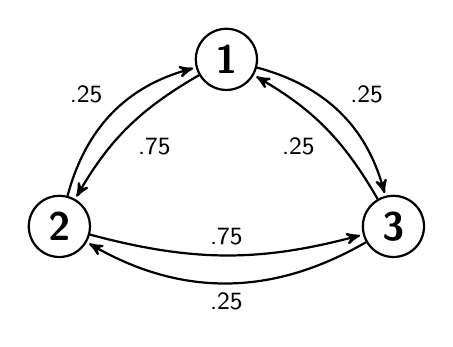
\begin{tikzpicture}[->,>=stealth',shorten >=1pt,on grid,auto,node distance=3cm,
  thick,main node/.style={circle,fill=white!20,draw,font=\sffamily\Large\bfseries}]

  \node[main node] (1) {1};
  \node[main node] (2) [below left of=1] {2};
  \node[main node] (3) [below right of=1] {3};

  \path[every node/.style={font=\sffamily\small}]
    (1) edge [bend right=15] node {.75} (2)
        edge [bend left=30]  node {.25} (3)
    (2) edge [bend left=30]  node {.25} (1)
        edge [bend right=15] node {.75} (3)
    (3) edge [bend left=30]  node {.25} (2)
        edge [bend right=15] node {.25} (1);
\end{tikzpicture}


\paragraph{Chapman-Kolmogorov Equation}  \label{chap-komo-eq-explain}
Let $P_{ij}^{(m)}$ be the m step transistion probability from state $i$ to $j$
defined as:
\begin{equation*} \begin{split}
	P_{ij}^{(m)} = P(X_{n+m} = j | X_n = i)
\end{split} \end{equation*}
To take m steps to go from (possibly visiting m in an intermediate state
multiple itmes), you can take m-1 to steps. At step m-1, you can arrive at any
state k. To go from each state k at the m-1 step to the m step, you just apply
the transisition probability.

We can sum the probabilities because the probabililites of going from state k in
the m-1 step to state j are mutually exclusive (they are mutually exclusive
because they are different states).

Lastly, we can mulitple the probability of going to state k in m-1 steps by the
probability of going to state j because the probabilities are independent.
\begin{equation*} \begin{split}
	P_{ij}^{(m)} = \sum_k p_{ik}^{(m-1)} p_{kj}
\end{split} \end{equation*}
Which is exactly the same as taking 1 step, and then m-1 steps.
\begin{equation*} \begin{split}
	P_{ij}^{(m)} = \sum_k p_{ik}p_{kj}^{(m-1)}
\end{split} \end{equation*}
For a derivation of this, see (\ref{chap-komo-eq-deriv}).


\paragraph{Irreducible Markov Chain} allows every state to be reached from every
other state for all pairs of states $i$ and $j$. More concretely:
\begin{equation*} \begin{split}
	\forall i \forall j \ne i : \exists m_{ij}  : P_{ij}^{(m_{ij})} > 0 
\end{split} \end{equation*}

\paragraph{Recurrent State}: State j is recurrent if after leaving state j then
you are guarenteed to eventually comeback.

Let $f_j^{(n)}$ be the probability that you first return to state j in n steps.

Notice that $f_j^{(0)} = 0$ because it's impossible to comeback without taking any
steps. Also notice that $f_j^{(1)} > 0$ is only possible is the transistion pointing
to itself $P_{jj} > 0$.

j is recurrent if and only if
\begin{equation*} \begin{split}
	f_j = \sum_{n=1}^\infty f_j^{(n)} = 1
\end{split} \end{equation*}

\paragraph{Recurrent Non-null} A state j is recurrent non-null if and only if we
get back to state j, but it does not take forever. More concretely: \\[0.5cm]
j is recurrent non-null if and only if j is recurrent ($f_j = 1$) and
\begin{equation*} \begin{split}
	M_j = \sum_{n=1}^\infty n f_j^{(n)}
\end{split} \end{equation*}
Where $M_j$ is the expected number of steps to come back.

\paragraph{Recurrent Null} j is recurrent null if and only if j is recurrent and
j is not recurrent non-null.


TODO EXAMPLE WITH DIAGRAM

TODO EXAMPLE WITH DIAGRAM

\paragraph{Periodicity} A state j is periodic if and only if the only way to
come back to state j is to take r, 2r, 3r, ... , cr, steps.  \\[0.5cm]

If a state j is not periodic, it's called aperiodic \\[0.5cm]

If state j as a self loop ($p_{jj} > 0$), then state j is aperiodic \\[0.5cm]

If the system is a irreducible Markov Chain, and contains a self loop, then all
states j are aperiodic.

\paragraph{State Probability} 
Let $X_n$ be the random variable for the state at interval n, then in a
homogeneous Markov Chain we have that:
\begin{equation*} \begin{split}
	\pi_j^{(n}) = P(X_n = j) \mbox{ - at step j }
\end{split} \end{equation*}
Let $p_{ij}$ be the transition probability for going from state $i$ to state $j$
(independant of time, so it's the same for all intervals ($X_n$), then
\begin{equation*} \begin{split}
	\pi_j^{(n+1)} = \sum_{i=0}^\infty p_{ij} \pi_i^{(n)}
	\mbox{ (by applying total probability)}
\end{split} \end{equation*}

Given initial conditions $\pi_j^{(0)} \forall j$, we can compute all
$\pi_j^{(i)}$ apply the above formula recursively.

\paragraph{Steady State Therom} (Equilibrium Probability Theorm) (I made up this name. It seems better
than 'Fundamental Theorm.)

If a homogeneous Markov Chain is irreducible and a periodic, then there exists a
limiting probability (equilibrium):
\begin{equation*} \begin{split}
	\pi_j = \lim_{n \to \infty} \pi_j^{(n)}
\end{split} \end{equation*}
which is independant of the initial conditions $\pi_j^{(0)}$. \\[0.5cm]

Moreover, if all states j are recurrent non-null, then $\pi_j$ is non zero and
can be uniquely etermined from the equations:
\begin{equation*} \begin{split}
	\pi_j = \sum_i p_{ij} \pi_i , \forall j
\end{split} \end{equation*}
\begin{equation*} \begin{split}
	\sum_j \pi_j = 1
\end{split} \end{equation*}

\subparagraph{Example}
\subparagraph*{}

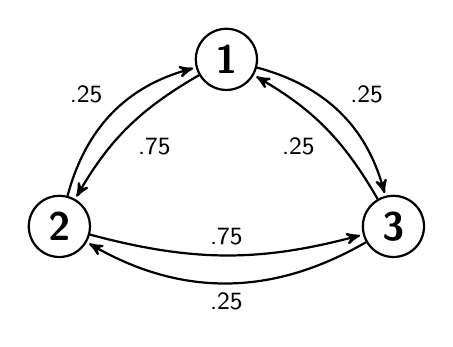
\begin{tikzpicture}[->,>=stealth',shorten >=1pt,on grid,auto,node distance=3cm,
  thick,main node/.style={circle,fill=white!20,draw,font=\sffamily\Large\bfseries}]

  \node[main node] (1) {1};
  \node[main node] (2) [below left of=1] {2};
  \node[main node] (3) [below right of=1] {3};

  \path[every node/.style={font=\sffamily\small}]
    (1) edge [bend right=15] node {.75} (2)
        edge [bend left=30]  node {.25} (3)
    (2) edge [bend left=30]  node {.25} (1)
        edge [bend right=15] node {.75} (3)
    (3) edge [bend left=30]  node {.25} (2)
        edge [bend right=15] node {.25} (1);
\end{tikzpicture}


\subparagraph*{}
Let the initial state be (1). This is the 'initial condition'

\subparagraph*{}
\begin{tabular}{ r | r  | r  |  r  |  r  |  r  |  r   | r }
	  n & 0 & 1  & 2  & 3  & 4  & ...  & $\infty$ \\
	\hline
	$\pi_1^{(n)}$ & 1 & 0    & .25   & .187  & .203  &  & .2 \\
	$\pi_2^{(n)}$ & 0 & .25  & .062  & .359  & .254  &  & .28 \\
	$\pi_3^{(n)}$ & 0 & .75  & .688  & .454  & .543  &  & .52 \\
\end{tabular}

\subparagraph*{}
To get the steady state column, you have to solve the system of equations that
results from the above theorm. From the table we can see that the emperical
basis for the steady state theorm. As you compute more columns, it approaches the values
computed from the steady state equations.


\paragraph{Residence Time in a State} The residence time, is the amount of time
that the system spends in state j for m steps, given that we are already in
state j.
\begin{equation*} \begin{split}
	P( \mbox{in state j for m steps} | \mbox{already in state j}) \\
	= P( \mbox{in state j for m steps} \wedge \mbox{step m+1 is not j} | \mbox{already in state j})
\end{split} \end{equation*}
We have that the transistion probabilities are independent of time
(homogeneous), so we can multiple the individual probabilities. $p_{jj}$ is the
homogeneous transistion probability of going from state j to state j.
\begin{equation*} \begin{split}
	= p_{jj}^m(1-p_{jj})
\end{split} \end{equation*}


\subsection{Continuous Time} In continuos time, state transistions happen
independtant of clock ticks. We can extend the discrete time theory we have
developed by considering the times $t_0$, $t_1$, $t_2$, ... , $t_n$. These are the
times when state transistions occur. \\[0.5cm]

Note that, if we can accept accuracy within a time interval, then we can just
use discrete time. Arrival and departure models generally use continuos time.
This distribution is heavily connected with the exponential function. \\[0.5cm]

\paragraph{Assumption: Continuos Time Markov Chain}
Let $X(t)$ be a random variable, where the distirbution of the random variable
depends on the real parameter t.
For instance, at $t=1.0$ the distribution of X
might be exponential, but at $t=\pi$ the distribution might be normal.
Given the above notation for state transistion, we have the following expression
for the probability of the $(n+1)^{th}$ state transistion.
\begin{equation*} \begin{split}
	P(X(t_{n+1}) = j | X(t_{n}) = i_n, ... ,  X(t_{0}) = i_0)
\end{split} \end{equation*}
Applying the Markov assumption that the next state transistion only depends on
the previous state gives us:
\begin{equation*} \begin{split}
	P(X(t_{n+1}) = j | X(t_{n}) = i_n)
\end{split} \end{equation*}

All the definitions we created in discrete time for recurrent, irreducible, etc
apply to continuos time as well by considering only the times when state
transistions occur.


\paragraph{Transistion Probability} Let the transistion probability be the
probability of going from one state i at time v, to another state at time t.
\begin{equation*} \begin{split}
	P_{ij}(v,t) = P(X(t)=j | X(v) = i)
\end{split} \end{equation*}
There is a special for the above formula:
\begin{equation*} 
	P_{ij}(t,t) =
	\begin{cases}
		1 \mbox{ if } i = j\\
		0 \mbox{ if } i \ne j
	\end{cases}
\end{equation*}


\paragraph{Apply Chapman-Kolmogorov Equation} We can apply the
Chapman-Kolmogorov Equation to the transistion probability. The probability of going
\begin{enumerate}
	\item from state i at time v
	\item to state j at time v
\end{enumerate}
is the same as going
\begin{enumerate}
	\item from state i at time v
	\item to state k at some intermediate time u (summed over all possible k's)
	\item to state j at time t 
\end{enumerate}
gives us the following equation:
\begin{equation*} \begin{split}
	P_{ij}(v,t) = \sum_{k=1}^\infty P_{ik}(v,u)P_{kj}(u,t)
\end{split} \end{equation*}
 
\paragraph{Partial of $P_{ij}(v,t)$} \label{pij-partial-derivation-context}
\begin{equation*} \begin{split}
	\frac{\partial P_{ij}(v,t)}{\partial t}
	= \lim_{\triangle t \to 0}
	\sum_{k \ne j} P_{ik}(v,t) \frac{P_{kj}(t,t+\triangle t)}{\triangle t}
		+ P_{ij}(v,t)\frac{P_{jj}(t,t+\triangle t) -1} {\triangle t}
\end{split} \end{equation*}
For a derivation of this, see (\ref{pij-partial-derivation}).

\paragraph{Rate Definitions for Simplificaiton} We define $q_{ij}$ in order to
simplify the partial expression above. Additionally, we define $q_{ij}$ in such
a way that $\sum_j q_{ij}(t) = 0  \forall i,t$
\begin{equation*} \begin{split}
	q_{kj}(t) = \lim_{\triangle t \to 0} \frac{P_{kj}(t,t+\triangle t)}{\triangle
	t} \mbox{ } k \ne j
\end{split} \end{equation*}
\begin{equation*} \begin{split}
	q_{jj}(t) = \lim_{\triangle t \to 0} \frac{P_{jj}(t,t+\triangle t)-1}{\triangle t}
\end{split} \end{equation*}
This gives us the intended simplication of the partial:
\begin{equation*} \begin{split}
	\frac{\partial P_{ij}(v,t)}{\partial t}
	= \lim_{\triangle t \to 0}
	\sum_{k \ne j} P_{ik}(v,t) q_{kj}(t)
	+ P_{ij}(v,t)q_{jj}(t)
\end{split} \end{equation*}
These $q_{ij}$'s become useful later on as they become the arrival and departure
rates in a birth-death process.


\paragraph{State Probabilitiy} \label{piej-derivative-derivation-context}
Let $\pi_j(t)$ be the probability of being in
state j, at time t.
\begin{equation*} \begin{split}
	\pi_j(t) = P(X(t) = j)
\end{split} \end{equation*}
By applying total probability, over some earlier time v we get:
\begin{equation*} \begin{split}
	\pi_j(t) = \sum_{i} P_{ij}(v,t) \pi_i(v) \mbox{ (which is identical to the discrete case)}
\end{split} \end{equation*}
Taking the derivative we arrive at (see derivation (\ref{piej-derivative-derivation})):
\begin{equation*} \begin{split}
	\frac{d \pi_j(t) }{dt} = \sum_{k\ ne j} \pi_k(t)q_{kj}(t) + \pi_j(t)q_{jj}(t)
\end{split} \end{equation*}
Applying the assumption that the transistion probabilities are homogeneous
(indepenant over time), we have that $q_{ij}(t) = q_{ij}$
\begin{equation*} \begin{split}
	\frac{d \pi_j(t) }{dt} = \sum_{k \ne j} \pi_k(t)q_{kj} + \pi_j(t)q_jj
\end{split} \end{equation*}

\paragraph{Steady State Results}

\paragraph{Residence Time in State}

\begin{equation*} \begin{split}
\end{split} \end{equation*}







\newpage
\section{Derivations}
\subsection{Probability}


\begin{equation*} \begin{split}
\end{split} \end{equation*}


\subsection{Stochastic Processes}


\paragraph{Chapman-Kolmogorov Equation} \label{chap-komo-eq-deriv}
For context see (\ref{chap-komo-eq-explain}).
TODO

\paragraph{Partial of $P_{ij}(v,t)$} \label{pij-partial-derivation}
For context see (\ref{pij-partial-derivation-context}).
TODO

\paragraph{Derivative of $\pi_j(t)$} \label{piej-derivative-derivation}
For context see (\ref{piej-derivative-derivation-context}).

\begin{equation*} \begin{split}
\end{split} \end{equation*}




\end{document}
